% -*- latex -*-
%%%%%%%%%%%%%%%%%%%%%%%%%%%%%%%%%%%%%%%%%%%%%%%%%%%%%%%%%%%%%%%%
%%%%%%%%%%%%%%%%%%%%%%%%%%%%%%%%%%%%%%%%%%%%%%%%%%%%%%%%%%%%%%%%
%%%%
%%%% This text file is part of the source of 
%%%% `The Art of HPC, vol 1: The Science of Computing'
%%%% by Victor Eijkhout, copyright 2012-2022
%%%%
%%%% This book is distributed under a Creative Commons Attribution 3.0
%%%% Unported (CC BY 3.0) license and made possible by funding from
%%%% The Saylor Foundation \url{http://www.saylor.org}.
%%%%
%%%%
%%%%%%%%%%%%%%%%%%%%%%%%%%%%%%%%%%%%%%%%%%%%%%%%%%%%%%%%%%%%%%%%
%%%%%%%%%%%%%%%%%%%%%%%%%%%%%%%%%%%%%%%%%%%%%%%%%%%%%%%%%%%%%%%%

The communication cost of this is
\begin{itemize}
\item $O(P)$ latency since messages need to be received from all processors.
\item $O(N)$ bandwidth, since all particles need to be received.
\end{itemize}
If we however distribute the force calculations, rather than the particles,
we come to different bounds; see~\cite{Driscoll:optimal-nbody} and
references cited therein.

With every processor computing the interactions in a block with sides $N/\sqrt P$, 
there is replication of particles and forces need to be collected.
Thus, the cost is now
\begin{itemize}
\item $O(\log p)$ latency for the broadcast and reduction
\item $O(N/\sqrt P\cdot \log P)$ bandwidth, since that is how much
  force data each processor contributes to the final sum.
\end{itemize}

\Level 2 {Problem description}

We abstract the N-body problem as follows:
\begin{itemize}
\item We assume that there is a vector~$c(\cdot)$
  of the particle charges/masses and location information. 
\item To compute the location update, we need the pairwise
  interactions $F(\cdot,\cdot)$ based on storing tuples
  $C_{ij}=\langle c_i,c_j\rangle$.
\item The interactions are then summed to a force vector~$f(\cdot)$.
\end{itemize}
In the \ac{IMP} model, the algorithm is sufficiently described 
if we know the respective data distributions; we are not immediately concerned with the 
local computations.

\Level 2 {Particle distribution}

\def\dottimes{\mathbin{\cdot_\times}}

An implementation based on particle distribution takes as its starting
point the particle vector~$c$ distributed as~$c(u)$, and
directly computes the force vector $f(u)$ on the same distribution.
We describe the
computation as a sequence of three kernels, two of data movement and
one of local computation\footnote{In the full \ac{IMP}
  theory~\cite{Eijkhout:ICCS2012} the first two kernels can be
  collapsed.}:
\begin{equation}
  \begin{cases}
    \{ \alpha\colon c(u) \}&\hbox{initial distribution for $c$ is $u$}\\
    C(u,*) = c(u)\dottimes c(*)&\hbox{replicate $c$ on each processor}\\
    \hbox{local computation of $F(u,*)$ from $C(u,*)$}\\
    f(u) = \sum_2 F(u,*)&\hbox{local reduction of partial forces}\\
    \hbox{particle position update}
  \end{cases}
  \label{eq:nbody-1d}
\end{equation}
The final kernel is a reduction with identical $\alpha$ and
$\beta$-distribution, so it does not involve data motion.
The local computation kernel also has not data motion.
That leaves the gathering of~$C(u,*)$ from the initial
distribution~$c(u)$. Absent any further information on the 
distribution~$u$ this is an allgather of $N$ elements,
at a cost of $\alpha\log p+\beta N$.
In particular, the communication cost does not go down
with~$p$.

With a suitable programming system based on distributions,
the system of equations~\eqref{eq:nbody-1d} can be
translated into code.

\Level 2 {Work distribution}

The particle distribution implementation used a one-dimensional
distribution $F(u,*)$ for the forces conformally with the particle
distribution. Since $F$~is a two-dimensional object, it is also
possible to use a two-dimensional distribution. We will now explore
this option, which was earlier described
in~\cite{Driscoll:optimal-nbody}; our purpose here is to show how this
strategy can be implemented and analyzed in the \ac{IMP} framework.
Rather than expressing the algorithm as
distributed computation and replicated data, we use a
distributed temporary, and we derive the replication scheme
as collectives on subcommunicators. 

For a two-dimensional distribution of~$F$ we need $(N/b)\times (N/b)$ processors
where $b$~is a blocksize parameter. For ease of exposition we use $b=1$,
giving a number of processors $P=N^2$.

We will now go through the necessary reasoning. The full algorithm in
close-to-implementable form is given in figure~\ref{fig:nbody-1.5d}.
\begin{figure}[t]
  \begin{equation}
    \begin{array}{ll}
      \{\alpha\colon C( D\colon <I,I>) \}&\hbox{initial distribution on the processor diagonal}\\
      C(I,I) = C(I,p)+C(q,I)&\hbox{row and column broadcast of the processor diagonal}\\
      F(I,I)\leftarrow C(I,I)&\hbox{local interaction calculation}\\
      f(D\colon<I,I>)=\sum_2 F(I,D\colon *)&\hbox{summation from row replication on the diagonal}
    \end{array}
    \label{eq:nbody-1.5d}
  \end{equation}
  \caption{IMP realization of the 1.5D N-body problem.}
  \label{fig:nbody-1.5d}
\end{figure}
For simplicity we use the identify distribution $I\colon p\mapsto\{p\}$.

\heading{Initial store on the diagonal of the processor grid}

\begin{wrapfigure}{r}{2in}
  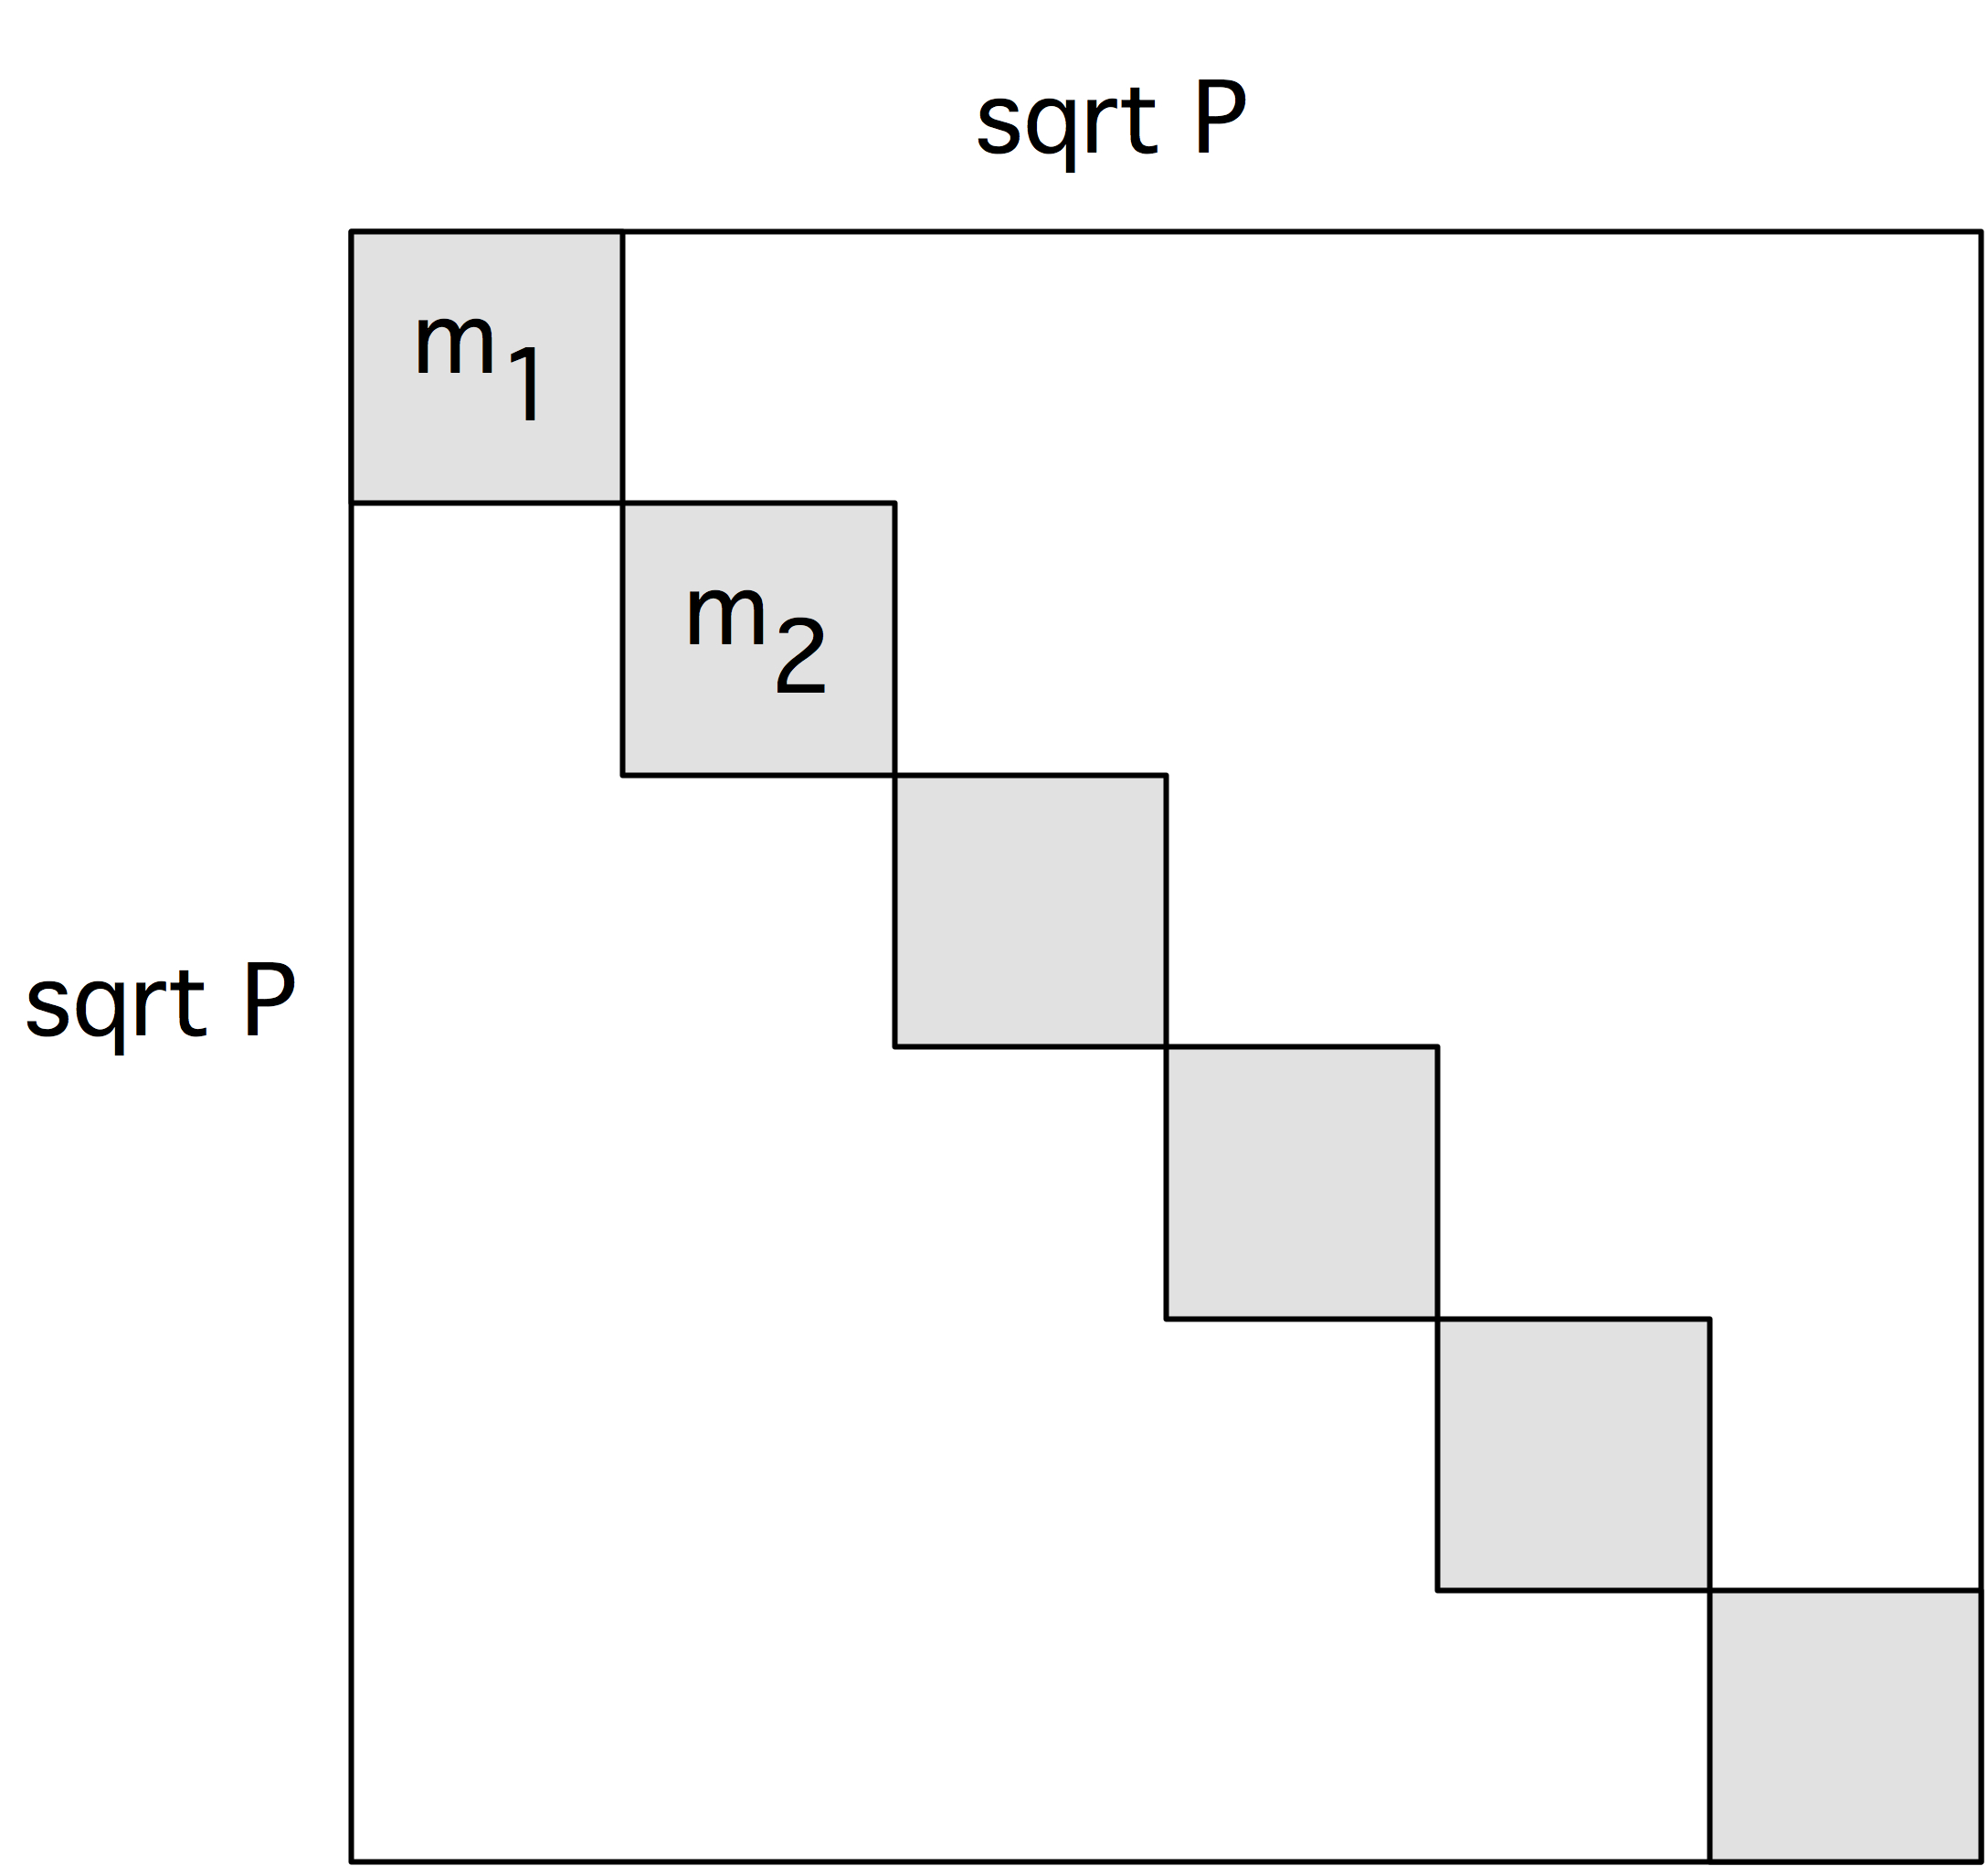
\includegraphics[scale=.06]{all-pairs-init}
\end{wrapfigure}
%
We first consider the gathering of the tuples $C_{ij}=\langle c_i,c_j\rangle$.
Initially, we decide to let the $c$~vector be stored on the diagonal of the processor grid;
in other words,
for all~$p$, processor~$\langle p,p\rangle$ contains~$C_{pp}$,
and the content of all other processors is undefined.

To express this formally, we let $D$ be the diagonal $\{\langle p,p\rangle\colon p\in P\}$.
Using the mechanism of partially defined distributions
the initial $\alpha$-distribution is then
\begin{equation}
C( D\colon <I,I>)\equiv D\ni \langle p,q\rangle\mapsto
C(I(p),I(q))=C_{pq}.
\label{eq:c-alpha}
\end{equation}

\heading{Replication for force computation}

\begin{wrapfigure}{r}{2in}
  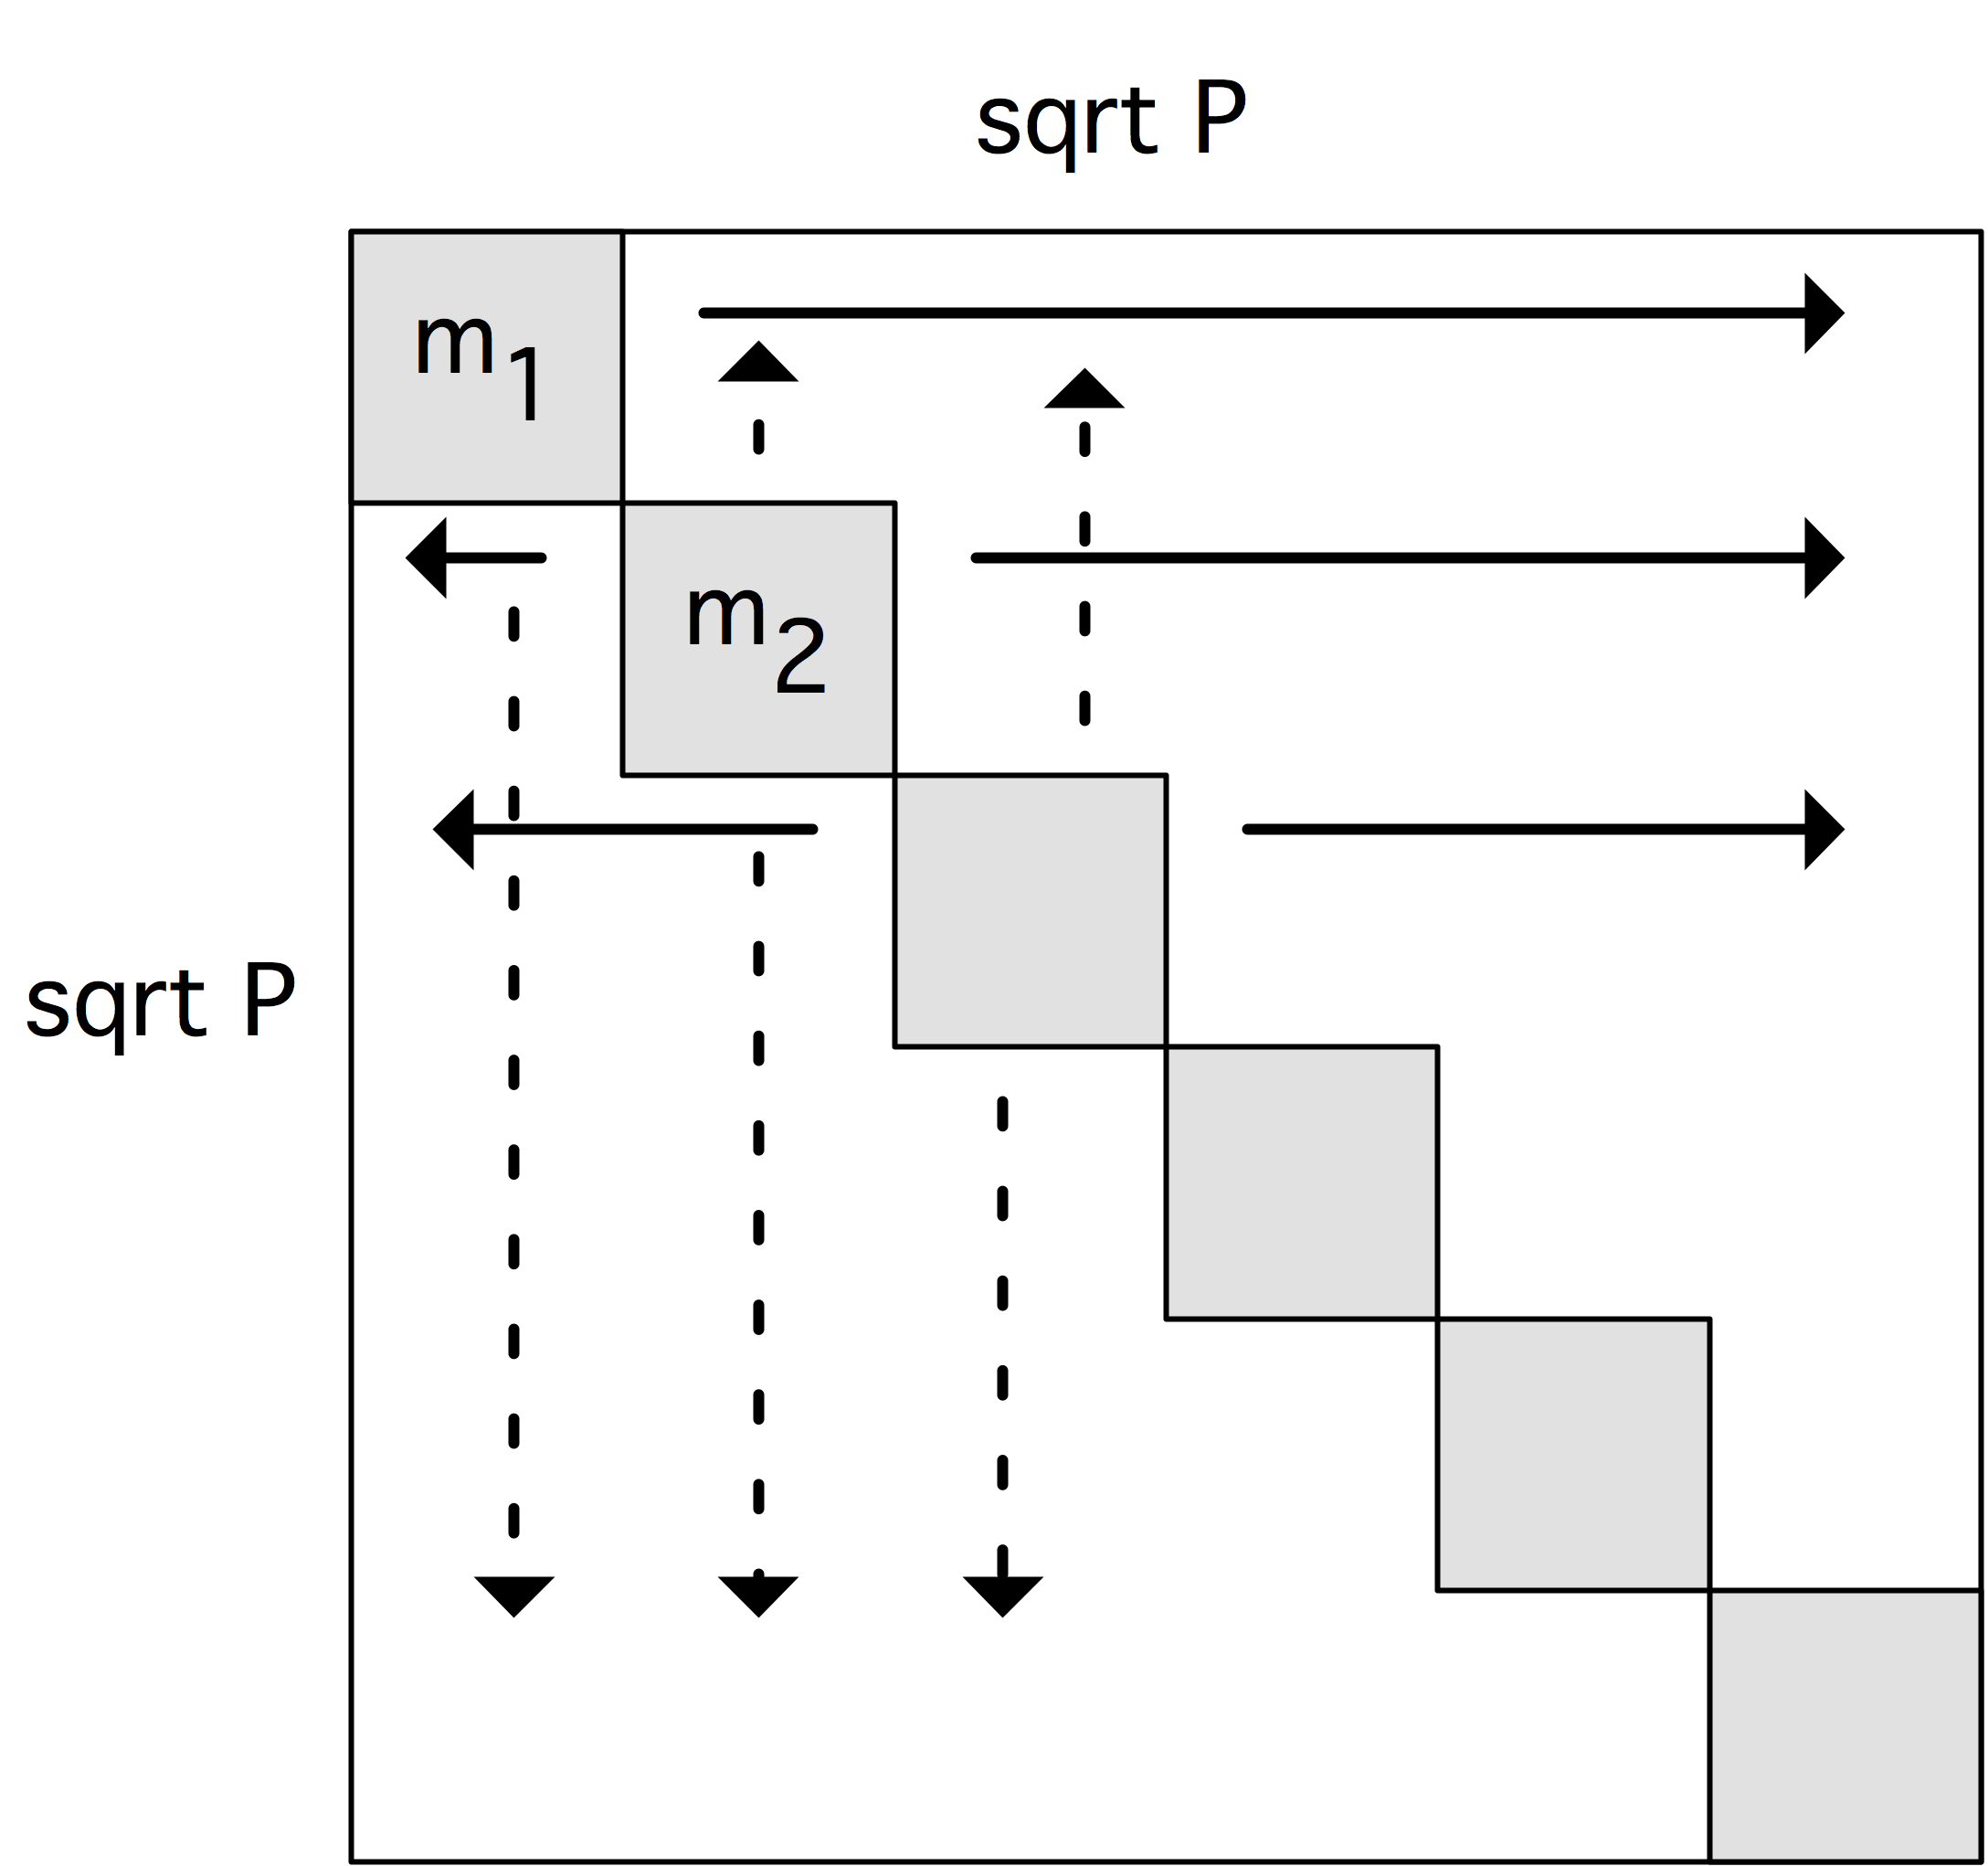
\includegraphics[scale=.06]{all-pairs-bcst}
\end{wrapfigure}
%
The local force computation $f_{pq}=f(C_{pq})$ needs for each processor $\langle p,q\rangle$
the quantity~$C_{pq}$, so we need a $\beta$-distribution of~$C(I,I)$.
The key to our story is the realization that 
\[ C_{pq} = C_{pp}+C_{qq} \]
so that
\[ C(I,I) = C(I,p)+C(q,I) \]
(where $p$ stands for the distribution that maps each processor
to the index value~$p$ and similarly for~$q$.)

To find the transformation from $\alpha$ to $\beta$-distribution
we consider the
transformation of the expression $C(D\colon\langle I,I\rangle)$.
In general, any set~$D$ can be written as a mapping from the first coordinate to
sets of values of the second:
\[ D\equiv p\mapsto D_p\qquad\hbox{where}\qquad
  D_p=\{q\colon \langle p,q\rangle\in D\}.
\]
In our particular case of the diagonal we have
\[ D\equiv p\mapsto\{p\}.\]
With this we write
\begin{equation}
C(D\colon \langle I,I\rangle) = C(I,D_p\colon I) = C(I,\{p\}\colon p).
\label{eq:c-alpha-rewrite}
\end{equation}

Note that equation~\eqref{eq:c-alpha-rewrite} is still the $\alpha$-distribution.
The $\beta$-distribution is $C(I,p)$, and it is an exercise in pattern matching to 
see that this is attained by a broadcast in each row, which carries a cost of
\[ \alpha \log\sqrt p + \beta N/\sqrt P. \]
Likewise, $C(q,I)$~is found from the $\alpha$-distribution by 
column broadcasts. We conclude that this variant does
have a communication cost that goes down proportionally
with the number of processors.

\heading{Local interaction calculation}

The calculation of $F(I,I)\leftarrow C(I,I)$ has identical $\alpha$ and $\beta$ 
distributions, so it is trivialy parallel.

\heading{Summing of the forces}

\begin{wrapfigure}{r}{2in}
  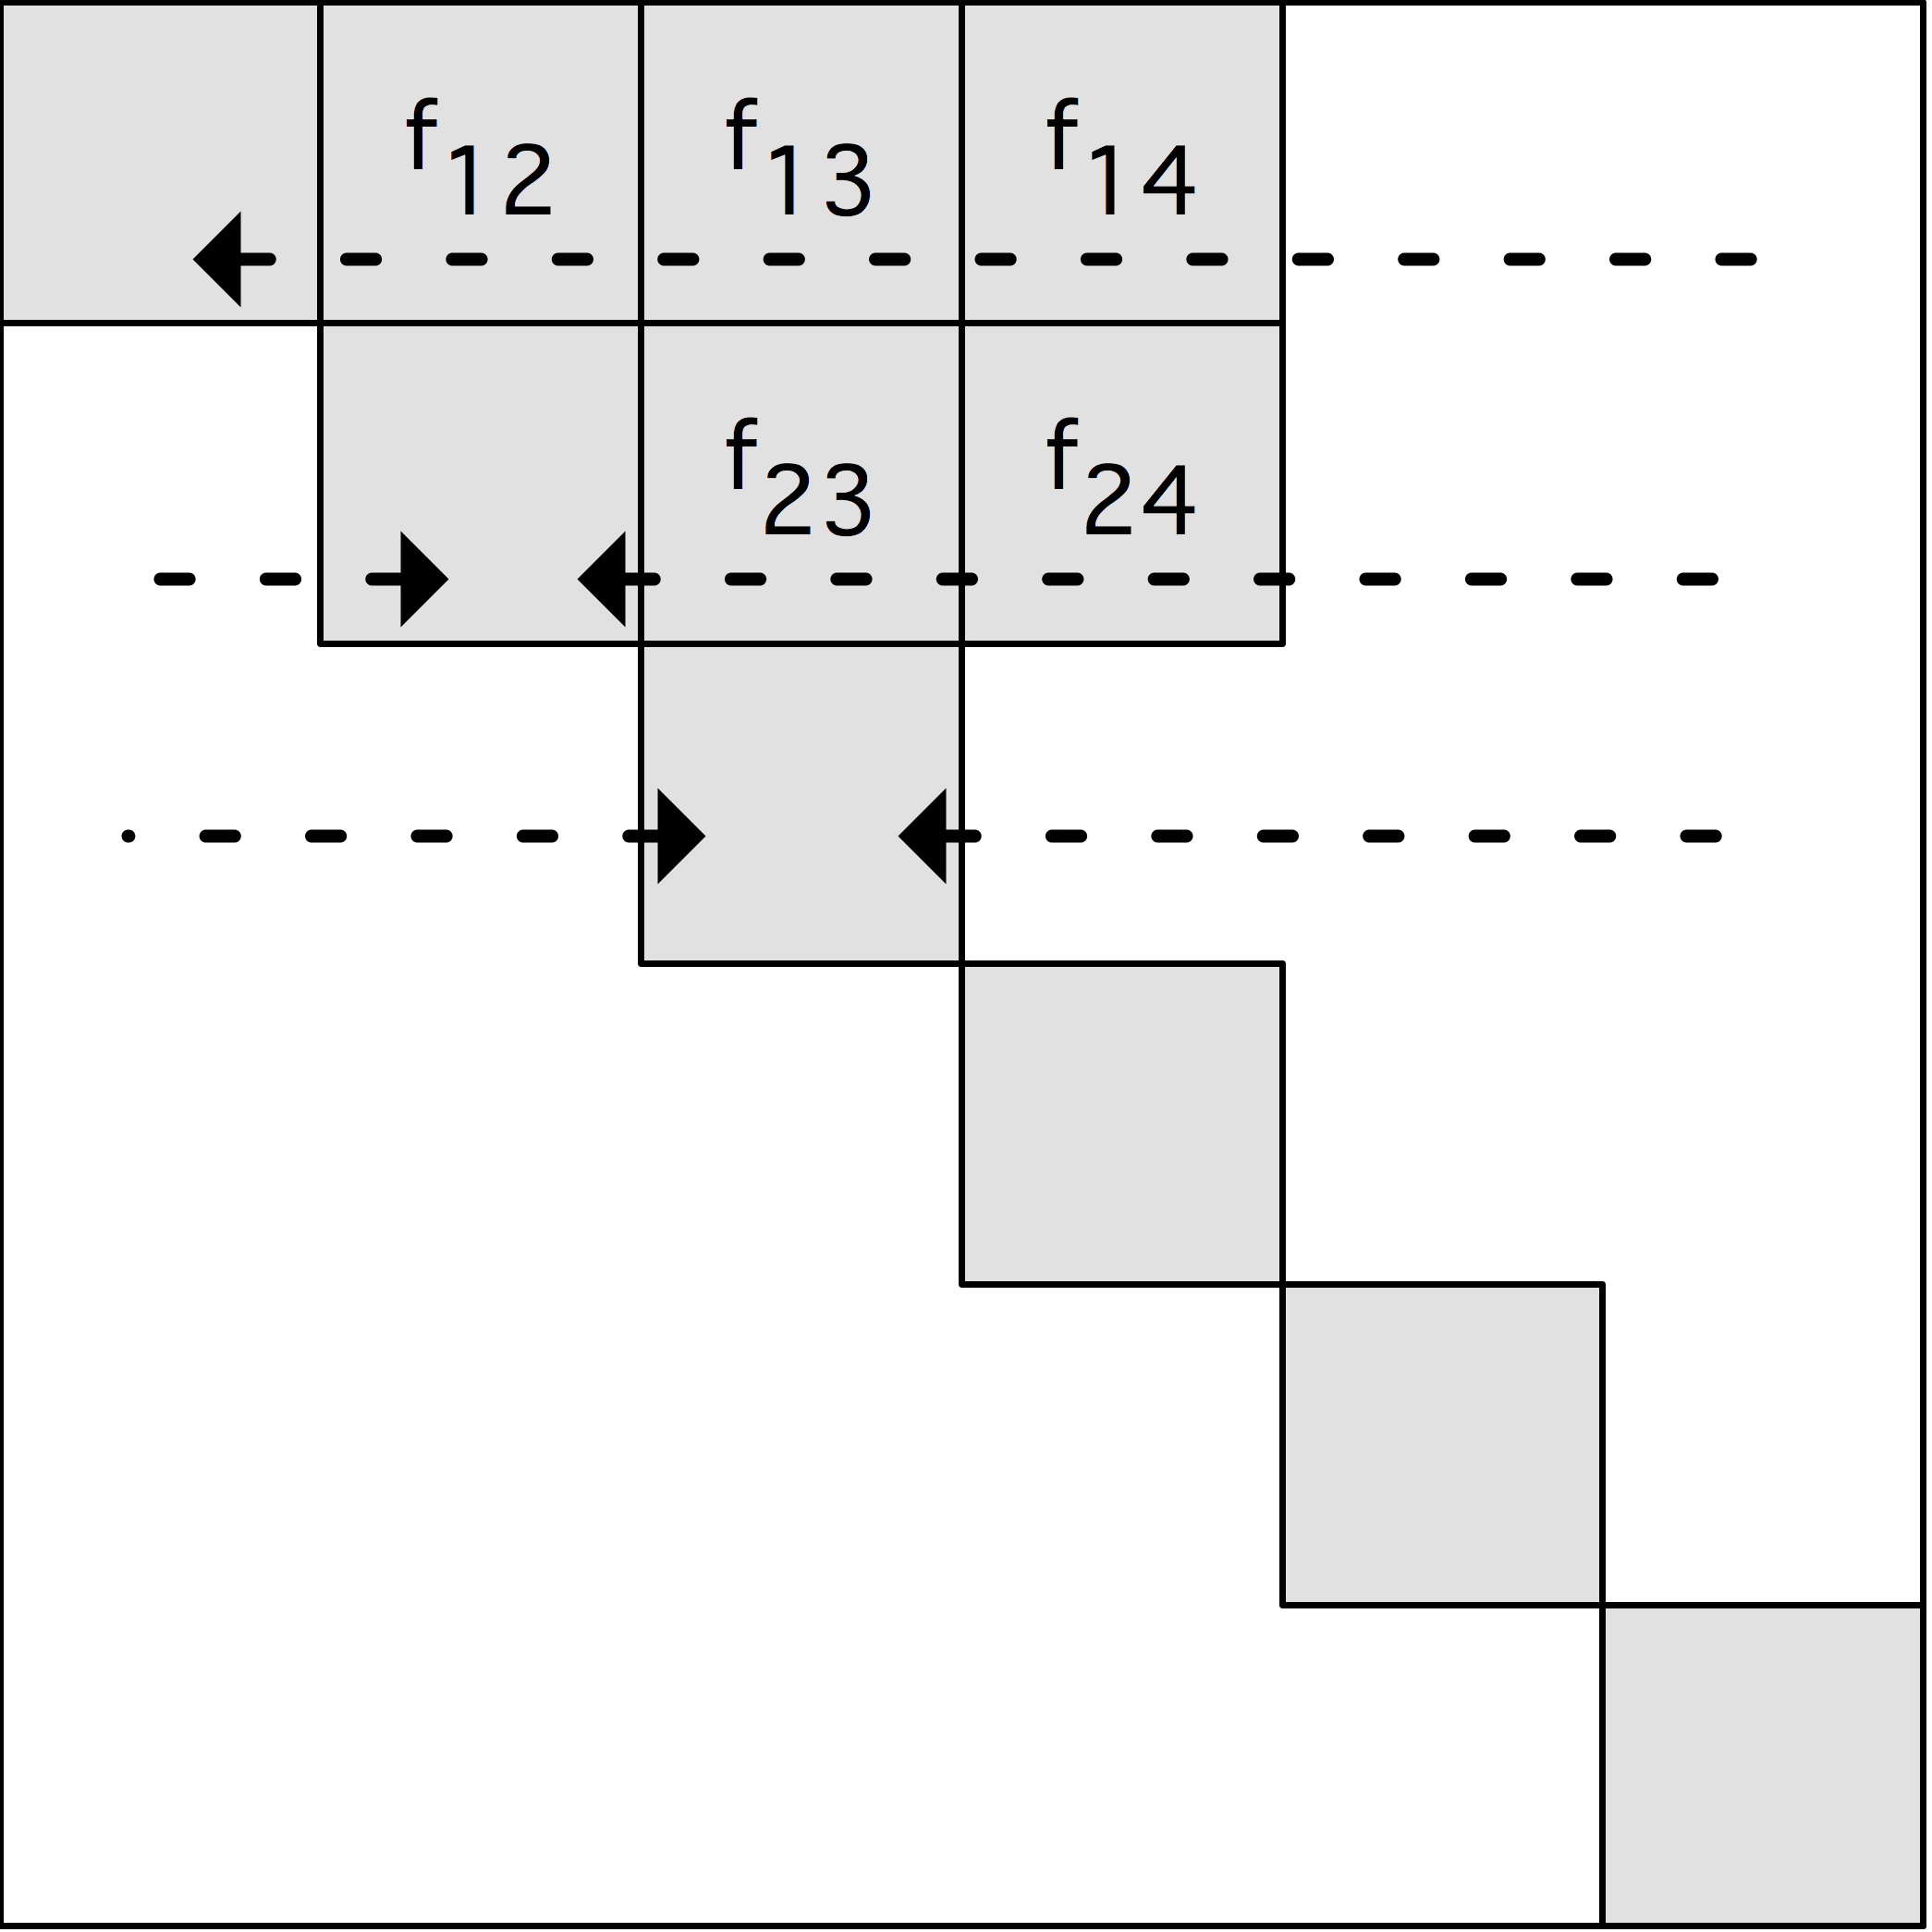
\includegraphics[scale=.06]{all-pairs-f}
\end{wrapfigure}
%
We have to extend the force vector~$f(\cdot)$ to our two-dimensional
processor grid as $f(\cdot,\cdot)$. However, conforming to the initial 
particle distribution on the diagonal, we only sum on the diagonal.
The instruction
\[ f(D\colon<I,I>)=\sum_2 F(I,D\colon *) \]
has a $\beta$-distribution of $I,D:*$, which is formed from the $\alpha$-distribution
of $I,I$ by gathering in the rows.

